%                      Code_Saturne version 1.3
%                      ------------------------
%
%     This file is part of the Code_Saturne Kernel, element of the
%     Code_Saturne CFD tool.
%
%     Copyright (C) 1998-2008 EDF S.A., France
%
%     contact: saturne-support@edf.fr
%
%     The Code_Saturne Kernel is free software; you can redistribute it
%     and/or modify it under the terms of the GNU General Public License
%     as published by the Free Software Foundation; either version 2 of
%     the License, or (at your option) any later version.
%
%     The Code_Saturne Kernel is distributed in the hope that it will be
%     useful, but WITHOUT ANY WARRANTY; without even the implied warranty
%     of MERCHANTABILITY or FITNESS FOR A PARTICULAR PURPOSE.  See the
%     GNU General Public License for more details.
%
%     You should have received a copy of the GNU General Public License
%     along with the Code_Saturne Kernel; if not, write to the
%     Free Software Foundation, Inc.,
%     51 Franklin St, Fifth Floor,
%     Boston, MA  02110-1301  USA
%
%-----------------------------------------------------------------------
\section{SOLUTION FOR CASE 2}
This case corresponds to a new study, in which there will be three calculation
cases (cases 2, 3 and 4). All of them can be created in a single {\itshape
cree\_sat} command, or additional cases can be added later. To test both
possibilities, first create the study directory, with cases directories CAS2
and CAS4:\\
{\itshape cree\_sat -etude FULL\_DOMAIN CAS2 CAS4}\\
then go in the study directory and add the CAS3 directory:\\
{\itshape cd FULL\_DOMAIN}\\
{\itshape cree\_sat -cas CAS3}

Go to the SCRIPT directory in CAS2,
open a new case and select the meshes to use. Click on the
item {\itshape Solution Domain}. In this case the three meshes have to be
pasted. So don't delete any mesh and activate the {\itshape Paste mesh} option by
clicking it {\itshape on}. Additional information appears on the page. If it is
left untouched, the \CS\ Preprocessor will test all the boundary faces for
potential pasting (based on geometrical criteria). To make mesh pasting more
efficient, this analysis can be restricted to a sub-set of boundary faces. This
is the case in the present calculation, since only faces of colors 5, 24 and 34
are liable to be pasted.

Click on the {\itshape Add} icon to enter the list of colors to be pasted.

\begin{figure}[h!]
\begin{center}
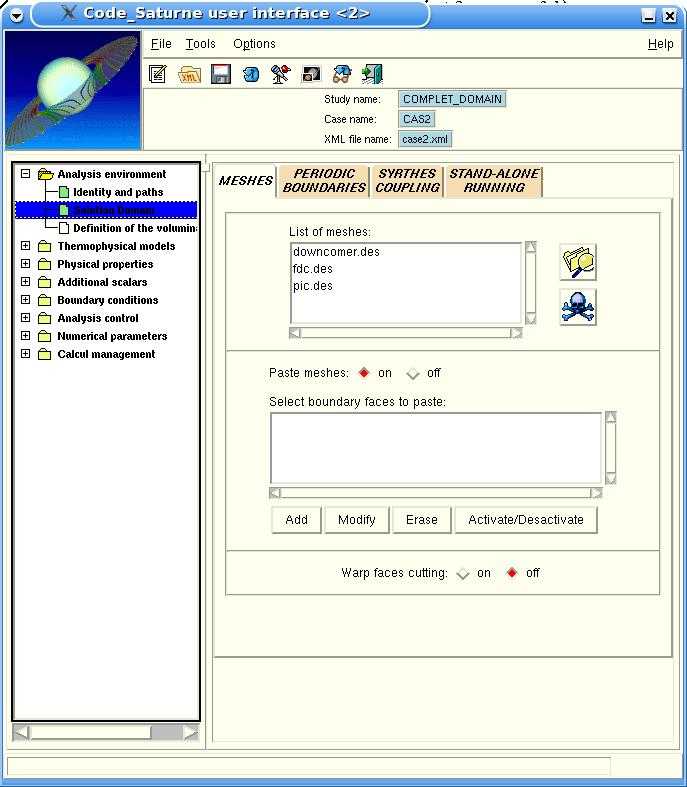
\includegraphics[width=12cm]{\repgraphics/c2_capture02.jpg}
\caption{Meshes: list of meshes}
\label{fig2_e2}
\end{center}
\end{figure}


\newpage
Clicking on {\itshape Add} opens a new window. Fill in the
{\itshape Input references} for the color reference to be pasted: 5, 24 and 32.
(different colors can be entered on a single line, separated by blanks). They
will appear in the area above. Then click on {\itshape Validate}.


\begin{figure}[h!]
\begin{center}
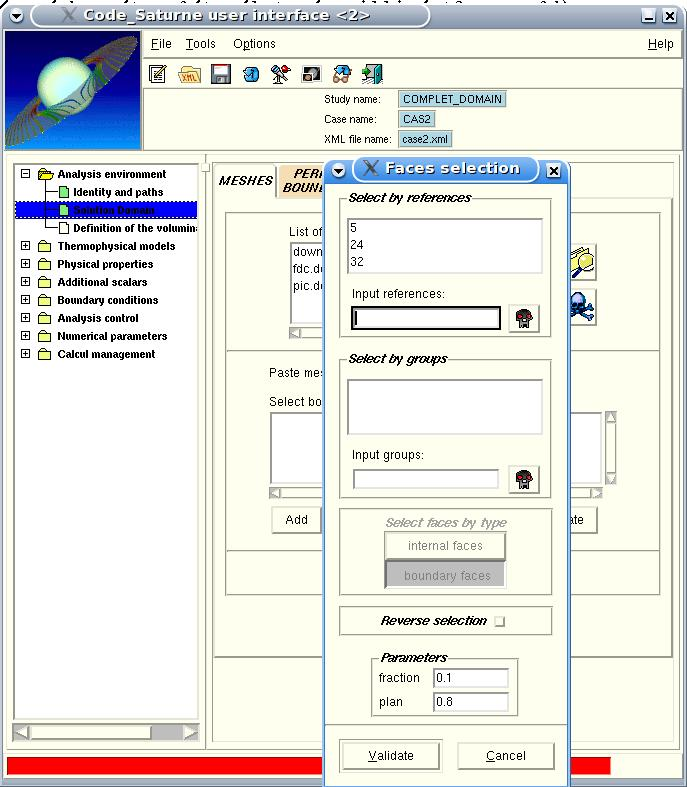
\includegraphics[width=12cm]{\repgraphics/c2_capture04.jpg}
\caption{Meshes: Join a mesh}
\label{fig4_e2}
\end{center}
\end{figure}


\newpage
The Preprocessor command for mesh pasting is now visible in the window (Fig
\ref{fig5_e2}). It will automatically be transfered into the launch script when
it is edited by the Interface.

\begin{figure}[h!]
\begin{center}
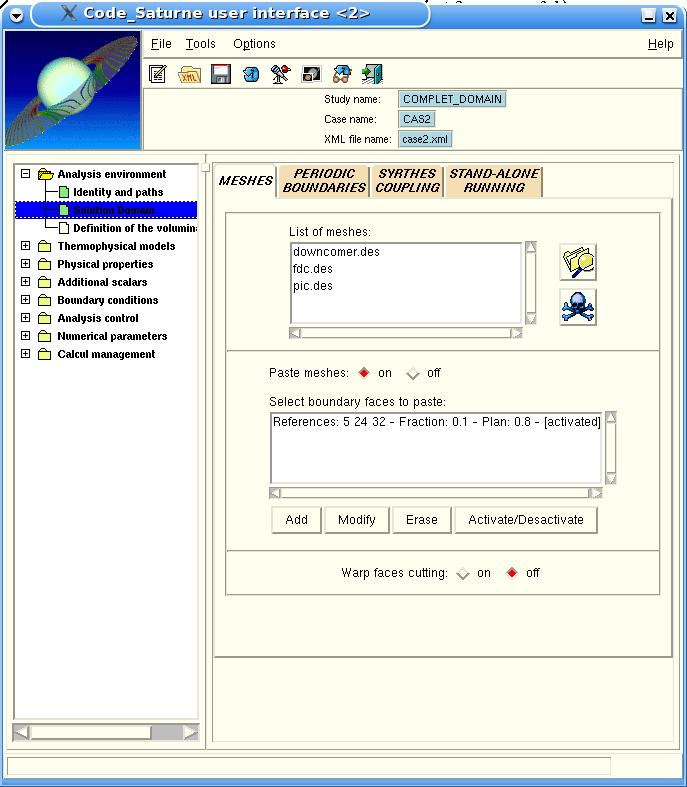
\includegraphics[width=12cm]{\repgraphics/c2_capture05.jpg}
\caption{Meshes}
\label{fig5_e2}
\end{center}
\end{figure}


\newpage
In this case ``Unsteady flow'' must be selected in the
{\itshape Analysis features} item.

\begin{figure}[h!]
\begin{center}
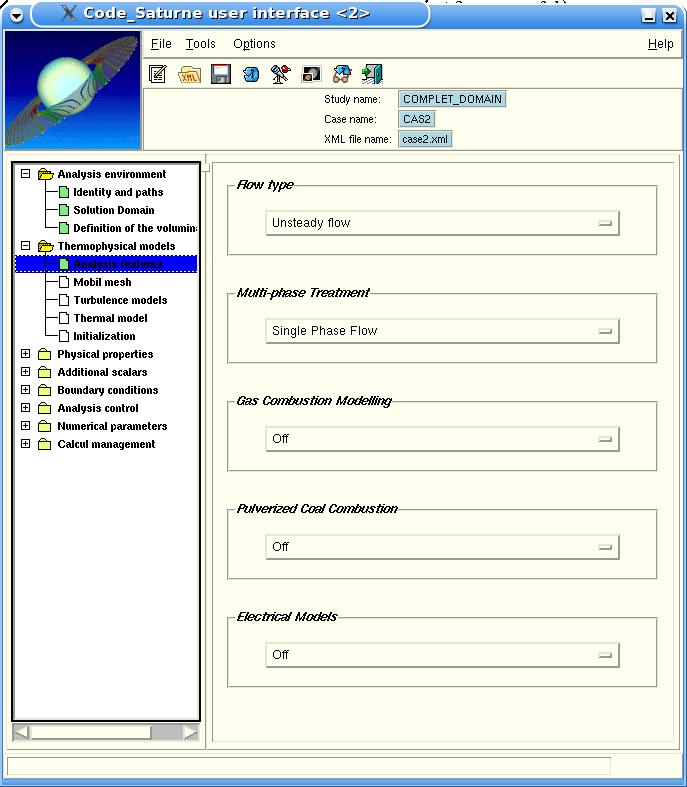
\includegraphics[width=12cm]{\repgraphics/c2_capture06.jpg}
\caption{Thermophysical models - Analysis features - Unsteady flow}
\label{fig6_e2}
\end{center}
\end{figure}

The rest of the heading {\itshape Thermophysical models} is identical to case
1.


\newpage
To add an additional scalar, click on the
{\itshape Definition and Initialization} item under the
{\itshape Additional scalars} heading.
The characteristics of the thermal scalar are still the
same. Its initial value is 20\degresC\ and it can vary between
0\degresC\ and 400\degresC.

To create an additional scalar, enter:\\
\hspace*{1cm}$\bullet\ $its {\itshape Name}: scalar\_2\\
\hspace*{1cm}$\bullet\ $its {\itshape Initial value}: 10\\
\hspace*{1cm}$\bullet\ $its {\itshape Minimal value}: 0\\
\hspace*{1cm}$\bullet\ $its {\itshape Maximal value}: 400

Then click on {\itshape Create}; the scalar will appear on the list,
below the thermal scalar.

\begin{figure}[h!]
\begin{center}
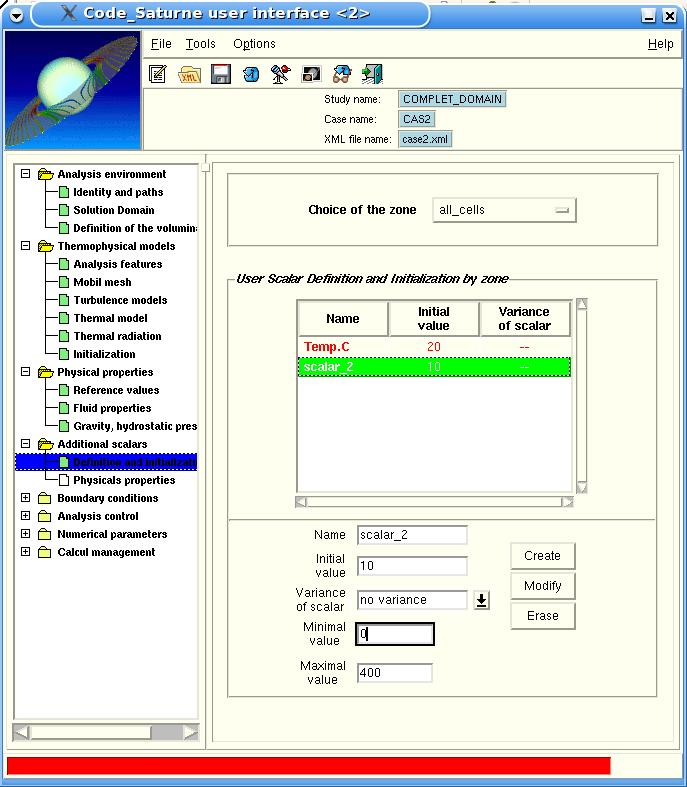
\includegraphics[width=12cm]{\repgraphics/c2_capture08.jpg}
\caption{Additional scalar - User scalar definition}
\label{fig8_e2}
\end{center}
\end{figure}


\newpage
In the item {\itshape Physical properties}, still under the heading
{\itshape Additional scalars}, specify the diffusion coefficient of this new
scalar. Click on the scalar name to highlight it, then enter the value in the
box. In this case, the value is
$0.895\times 10^{-4}\ m^{2}.s^{-1}$

\begin{figure}[h!]
\begin{center}
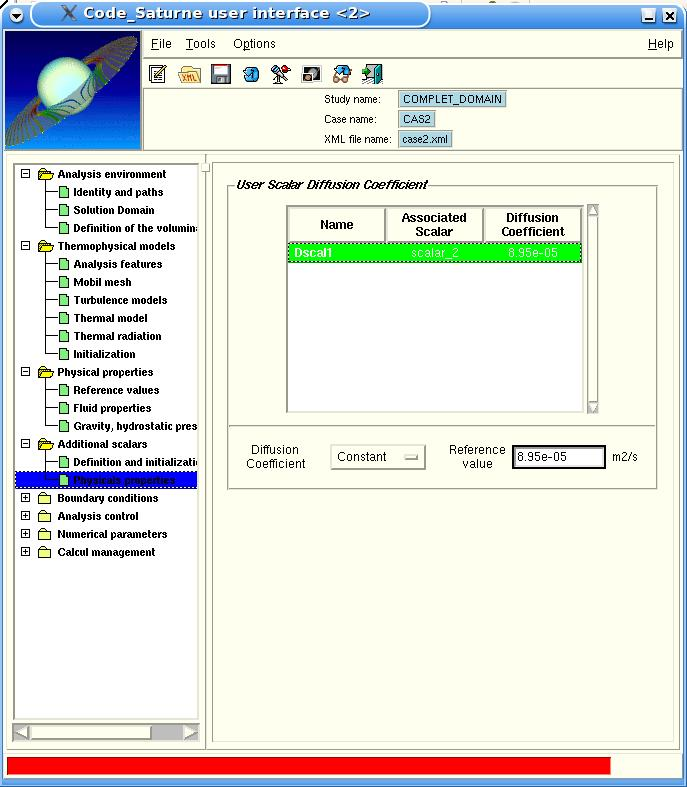
\includegraphics[width=12cm]{\repgraphics/c2_capture09.jpg}
\caption{Additional scalar - User scalar physical properties}
\label{fig9_e2}
\end{center}
\end{figure}


\newpage
Create the boundary zones. The procedure is the same as in case 1, but the
colors are different. Note that colors 5 and 32 have completely disappeared in
the pasting process (they are now internal faces and are not considered as
boundaries), while some boundary faces of color 24 remain.\\
Create the inlet, outlet
and symmetry boundary zones with the following colors:\\
\hspace*{1cm}$\bullet\ $inlet: color 1\\
\hspace*{1cm}$\bullet\ $outlet: color 34\\
\hspace*{1cm}$\bullet\ $symmetry: colors 8 9 28 29 38 39\\

\begin{figure}[h!]
\begin{center}
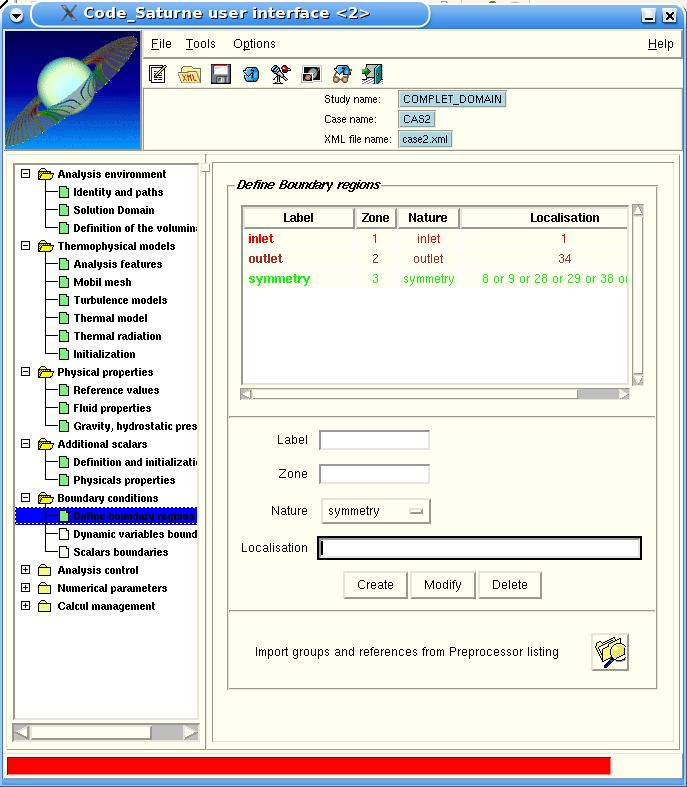
\includegraphics[width=12cm]{\repgraphics/c2_capture10.jpg}
\caption{Creation of the boundary zones}
\label{fig10_e2}
\end{center}
\end{figure}


\newpage
In this case, different conditions are applied for the walls. Separate
corresponding wall boundary regions must therefore be created, following the
data in the following table.

\begin{center}
\begin{tabular}{cccc}
Label & Zone & Nature & Localization \\
wall\_2 & 5 & wall & 2 or 3 \\
wall\_3 & 6 & wall & 4 or 7 or 21 or 22 or 23 \\
wall\_4 & 7 & wall & 6 and Y$>$1 \\
wall\_5 & 8 & wall & 6 and Y$\leqslant$1 \\
wall\_6 & 9 & wall & 31 or 33 \\
\end{tabular}
\end{center}

The ``wall\_1'' region combines color and geometrical criteria. The associated
character string to enter in the ``Localization'' box is as follows:\\
``24 and 0.1$<$=X and 0.5$>$=X''\footnote{Note that, due to the pasting process,
there are in fact no boundary faces of color 24 with X coordinate outside the
[0.1;0.5] intervalle. The geometrical criterium is therefore not
necessary. It is presented here to show the capacity of the face selection
module}.

\begin{figure}[h!]
\begin{center}
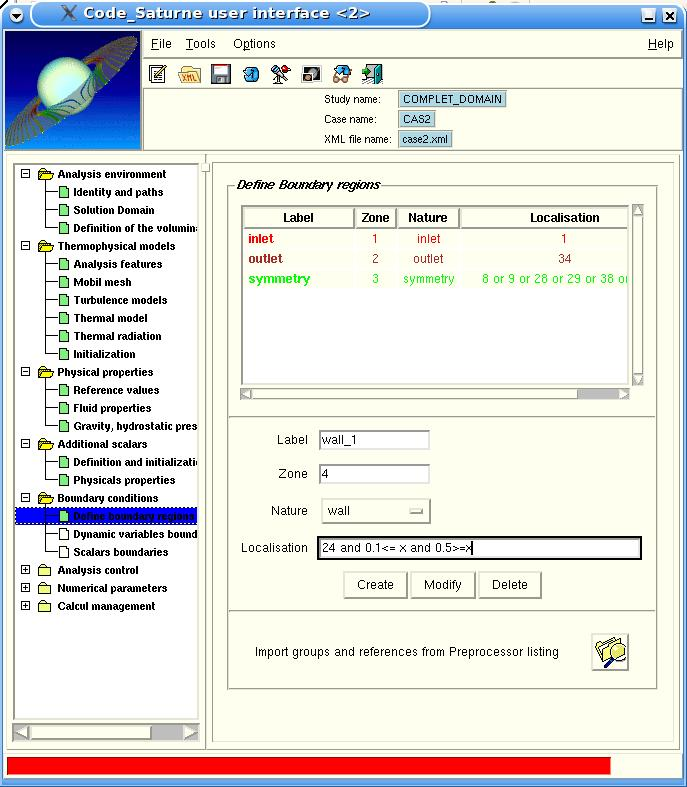
\includegraphics[width=12cm]{\repgraphics/c2_capture11.jpg}
\caption{Creation of a wall boundary region}
\label{fig11_e2}
\end{center}
\end{figure}


\newpage
Define the other wall boundary zones. The faces of color 6 have to be divided in
two separate zones, based on a geometrical criterium on $Y$.

\begin{figure}[h!]
\begin{center}
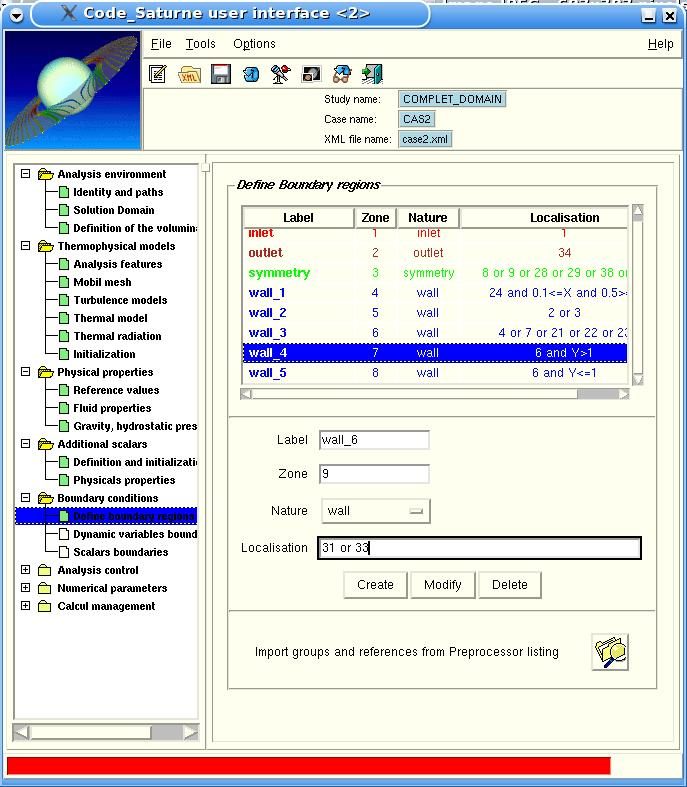
\includegraphics[width=12cm]{\repgraphics/c2_capture152.jpg}
\caption{Creation of wall boundary regions}
\label{fig152_e2}
\end{center}
\end{figure}


\newpage
The dynamic boundary conditions are the same as in case 1 for the inlet, and
there are still no sliding walls.


\begin{figure}[h!]
\begin{center}
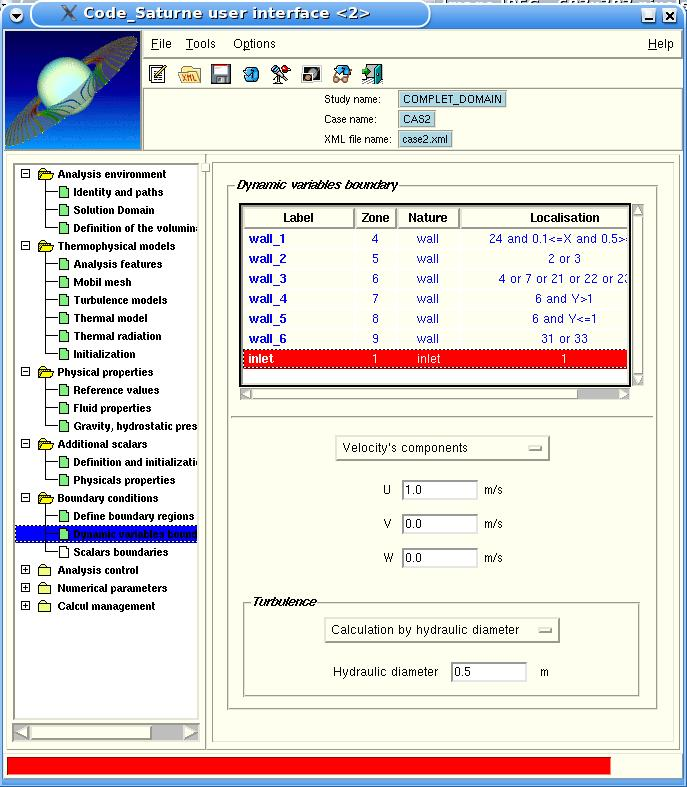
\includegraphics[width=12cm]{\repgraphics/c2_capture16.jpg}
\caption{Dynamic variables boundary: inlet}
\label{fig16_e2}
\end{center}
\end{figure}


\newpage
To configure the scalar boundary conditions, click on the item
{\itshape Scalars boundaries}.
On all the walls, a default homogeneous Neumann condition is set for
temperature, and Dirichlet conditions are specified for the passive scalar,
according to the following table:
\begin{center}
\begin{tabular}{|c|c|c|}
\hline
Wall & Nature & Value \\
\hline
wall\_1 & Dirichlet  & 0 \\
\hline
wall\_2 & Dirichlet  & 5 \\
\hline
wall\_3 & Dirichlet  & 0 \\
\hline
wall\_4 & Dirichlet  & 25 \\
\hline
wall\_5 & Dirichlet  & 320 \\
\hline
wall\_6 & Dirichlet  & 40 \\
\hline
\end{tabular}
\end{center}

\begin{figure}[h!]
\begin{center}
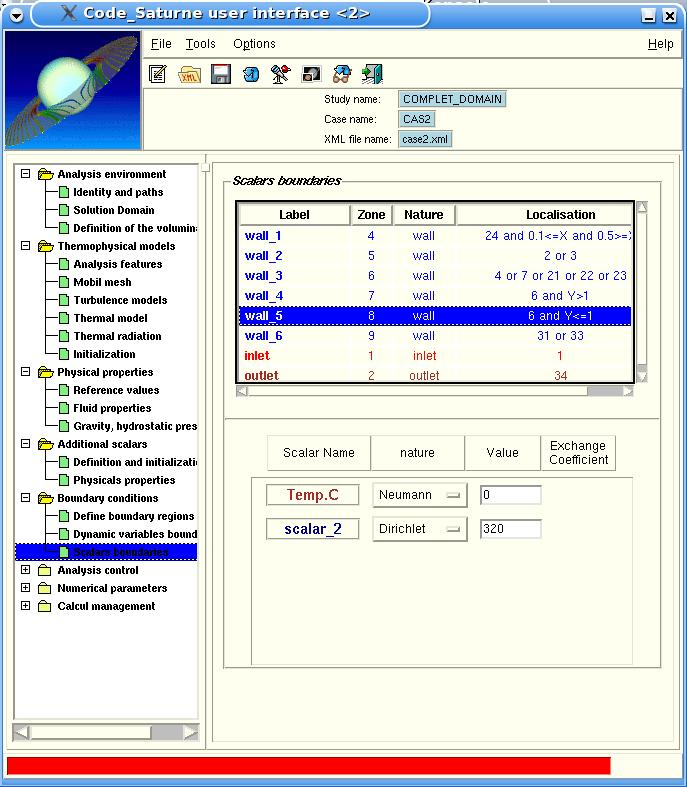
\includegraphics[width=12cm]{\repgraphics/c2_capture21.jpg}
\caption{Scalars boundaries: wall\_5}
\label{fig21_e2}
\end{center}
\end{figure}


\newpage
Click on {\itshape inlet}, to set the inlet values for the scalars: 300\degresC\
for temperature and 200 for the passive scalar.

\begin{figure}[h!]
\begin{center}
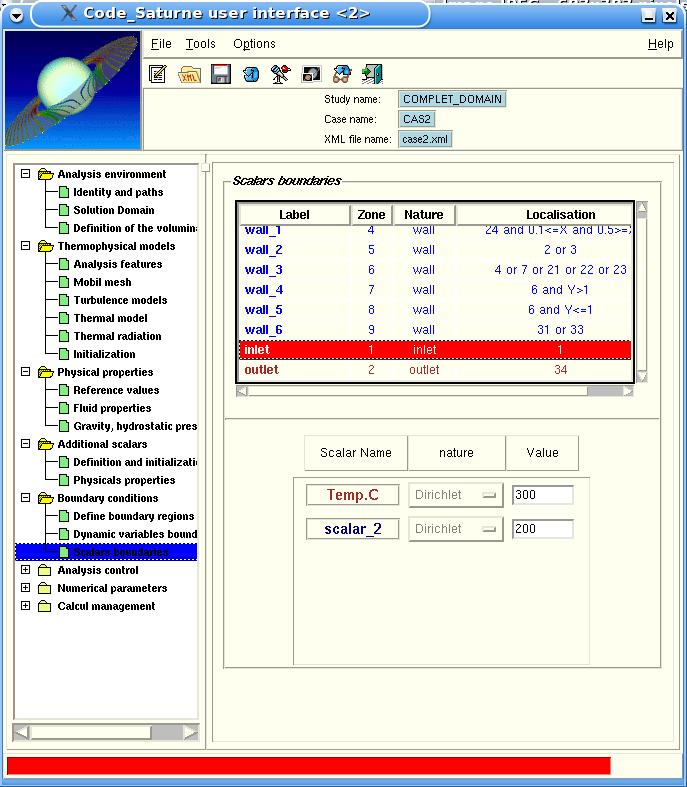
\includegraphics[width=12cm]{\repgraphics/c2_capture22.jpg}
\caption{Scalars boundaries: inlet}
\label{fig22_e2}
\end{center}
\end{figure}


\newpage
Some calculation parameters now need to be defined.
Go to the item {\itshape Time step} under the heading
{\itshape Analysis control}. In our case the time step is
{\itshape Uniform and constant}. Set the number of iterations to 300 and the
reference time step to $0.05\ s$.

\begin{figure}[h!]
\begin{center}
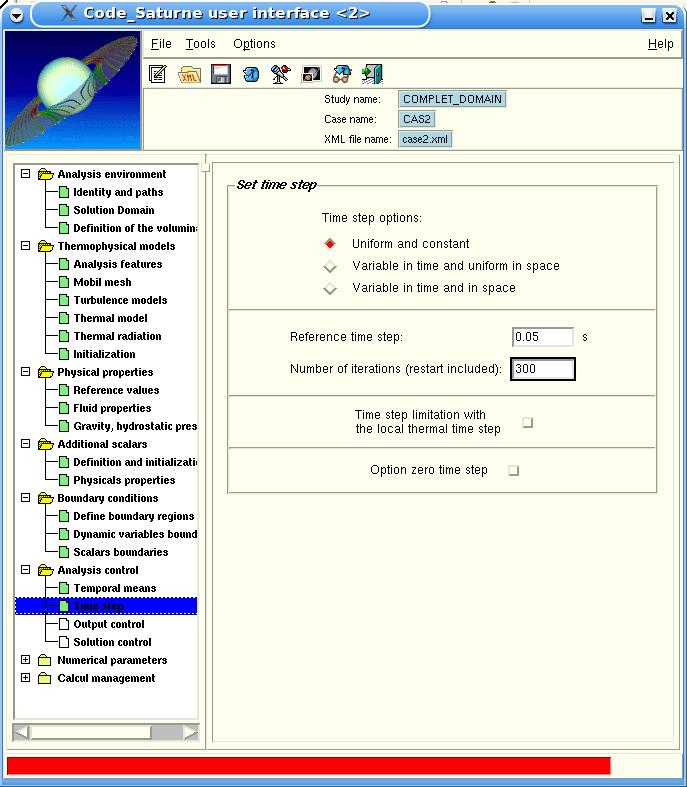
\includegraphics[width=12cm]{\repgraphics/c2_capture23.jpg}
\caption{Time step setting}
\label{fig23_e2}
\end{center}
\end{figure}


\newpage
Go to the item {\itshape Output control} to set the output parameters.

Keep the default value for the output listing frequency.

For the Post-processing, select the second option (output every 'n' time steps)
and set the value of 'n' to 2.

Activate the post-processing on the boundary faces by ticking the
{\itshape Domain boundary post processing} box. The EnSight format file will
contain an additional part, composed of the boundary faces, on which boundary
conditions and some other variables can be visualized. This allows to check if
the boundary conditions for the passive scalar have been properly set.

\begin{figure}[h!]
\begin{center}
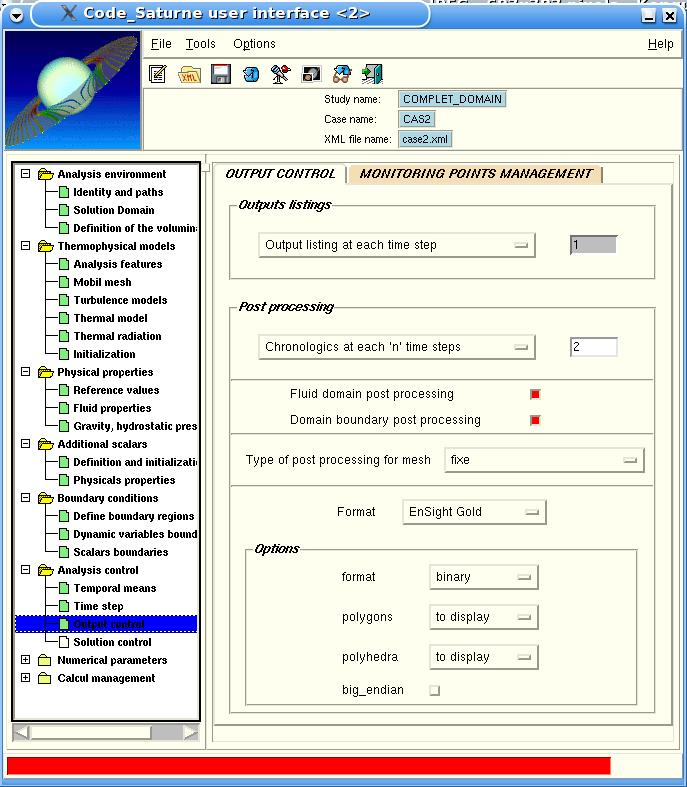
\includegraphics[width=12cm]{\repgraphics/c2_capture24.jpg}
\caption{Output control: post-processing}
\label{fig24_e2}
\end{center}
\end{figure}


\newpage
In this case, chronological records on specified monitoring probes are needed.
To define the probes, click on the
{\itshape Monitoring points management} tab.

\begin{figure}[h!]
\begin{center}
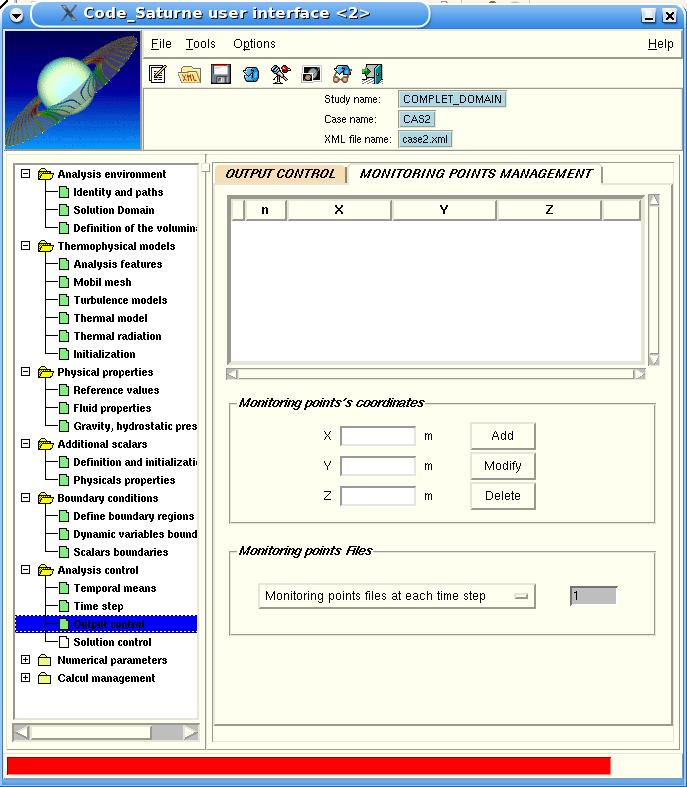
\includegraphics[width=12cm]{\repgraphics/c2_capture25.jpg}
\caption{Output control: monitoring points}
\label{fig25_e2}
\end{center}
\end{figure}



\newpage
Enter the coordinates of the monitoring points you want to define. For the first point:\\
\hspace*{1cm}$\bullet\ X = -0.25\ m$\\
\hspace*{1cm}$\bullet\ Y = 2.25\ m$\\
\hspace*{1cm}$\bullet\ Z = 0\ m$

\begin{figure}[h!]
\begin{center}
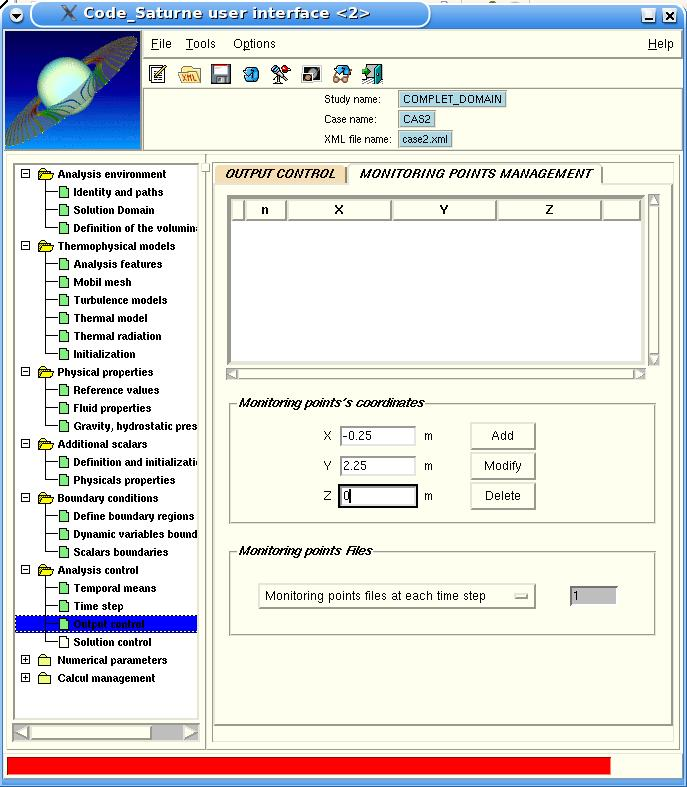
\includegraphics[width=12cm]{\repgraphics/c2_capture26.jpg}
\caption{Output controls: monitoring points - $1^{st}$ point}
\label{fig26_e2}
\end{center}
\end{figure}


\newpage
Then click on the {\itshape Add} button. The newly created point will appear in
the window above.

\begin{figure}[h!]
\begin{center}
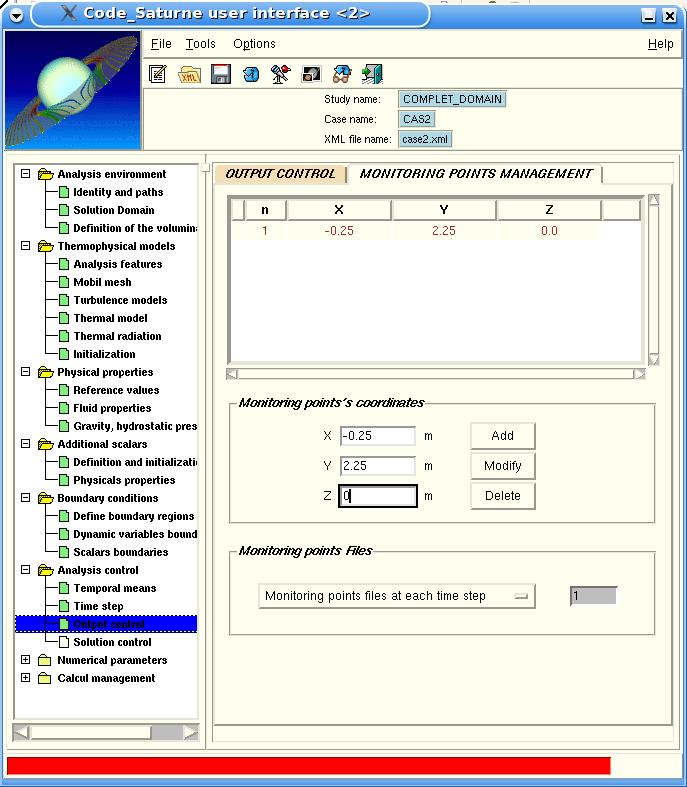
\includegraphics[width=12cm]{\repgraphics/c2_capture27.jpg}
\caption{Output controls: monitoring points - $1^{st}$ point}
\label{fig27_e2}
\end{center}
\end{figure}


\newpage
Repeat the procedure for the other probes. Their coordinates are indicated in
the following table (the Z coordinate is always 0).
\begin{center}
\begin{tabular}{|c|c|c|}
\hline
Points & X(m) & Y(m) \\
\hline
2 & 0.05 & 2.25 \\
\hline
3 & 0.05 & 2.75 \\
\hline
4 & 0.05 & 0.5 \\
\hline
5 & 0.05 & -0.25 \\
\hline
6 & 0.75 & -0.25 \\
\hline
7 & 0.75 & 0.25 \\
\hline
8 & 0.75 & 0.75 \\
\hline
\end{tabular}
\end{center}

\begin{figure}[h!]
\begin{center}
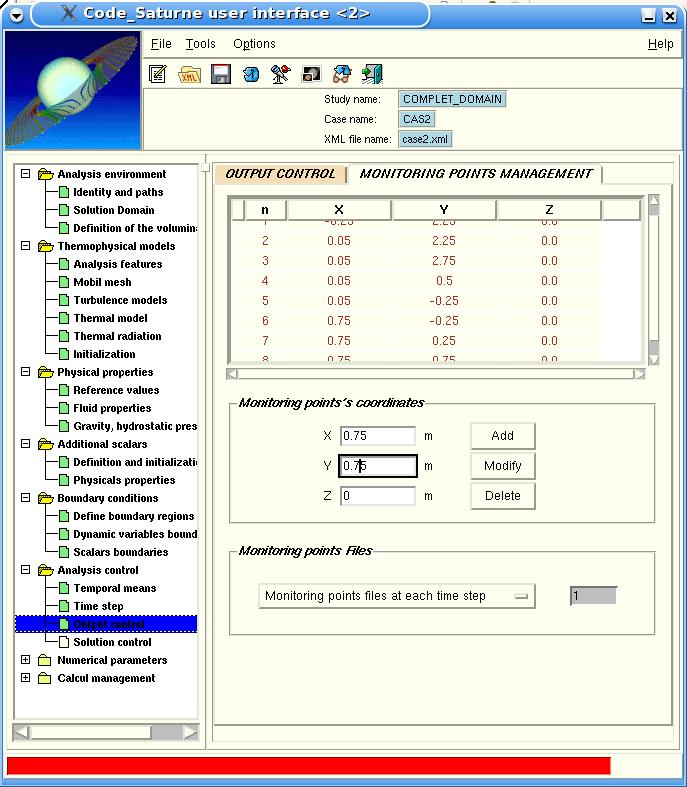
\includegraphics[width=12cm]{\repgraphics/c2_capture28.jpg}
\caption{Output control: monitoring points}
\label{fig28_e2}
\end{center}
\end{figure}

Remember to save the Xml file regularly.


\newpage
Go to the item {\itshape Solution control} to define which variables will
appear in the listing, the post-processing and the chronological records.

Uncheck the boxes in front of the {\itshape Pressure}, {\itshape Tubulent energy}
and {\itshape Dissipation} variables, in the {\itshape  Print in listing}
column. Information on these three variables will not appear in the output
listing anymore.

Uncheck the boxes in front of the {\itshape Courant number} and {\itshape
Fourier number} variables in the {\itshape Post-processing} column. These
variables will be removed from the post-processing results.

\begin{figure}[h!]
\begin{center}
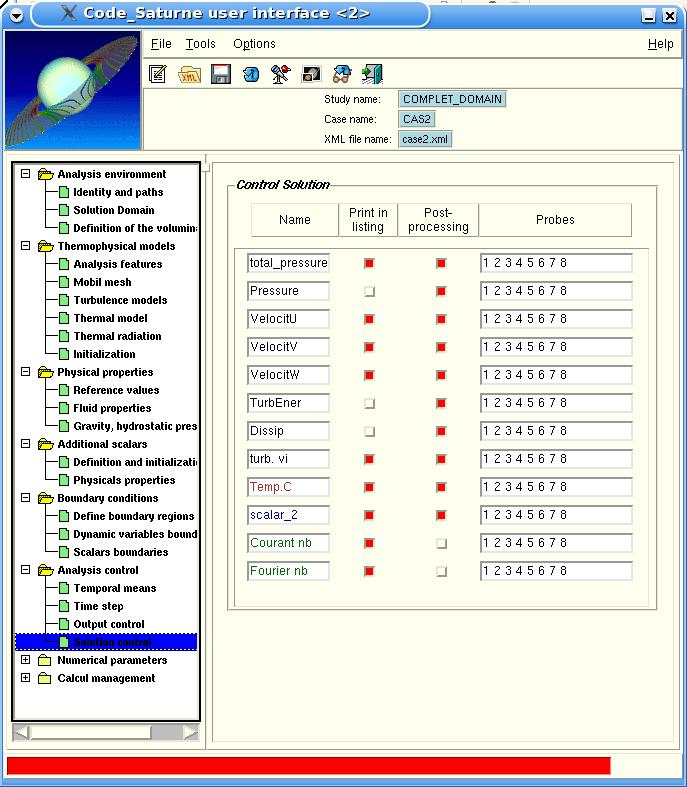
\includegraphics[width=12cm]{\repgraphics/c2_capture29.jpg}
\caption{Solution control - Output configuration}
\label{fig29_e2}
\end{center}
\end{figure}


\newpage
Delete all the probe numbers for the {\itshape total\_pressure} variable. No
chronological record will be created for this variable. As for the
{\itshape VelocitU} variable, only select probes  1, 2, 6, 7 and 8. Time
evolution on the other probes will not be recorded.

\begin{figure}[h!]
\begin{center}
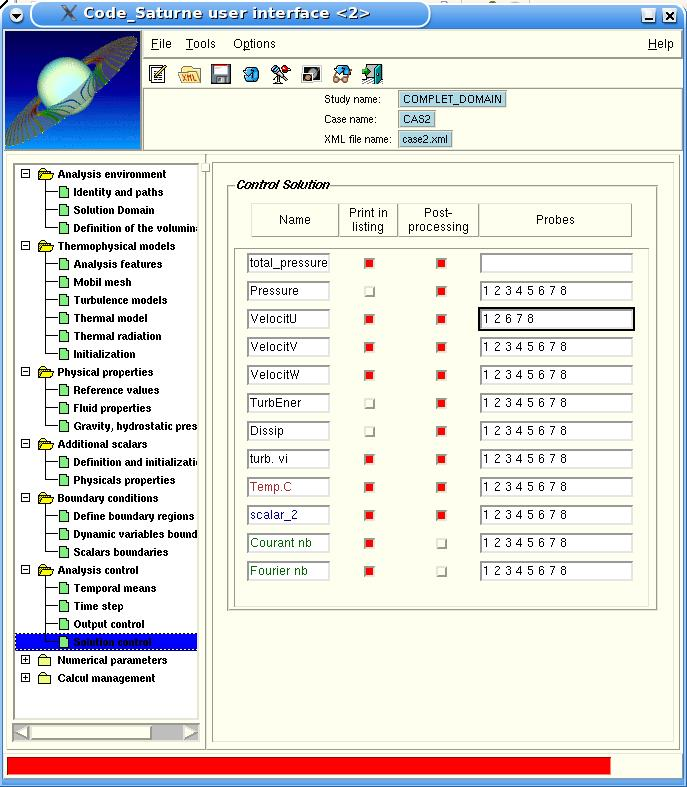
\includegraphics[width=12cm]{\repgraphics/c2_capture30.jpg}
\caption{Solution control - Probes}
\label{fig30_e2}
\end{center}
\end{figure}


No change is needed under the {\itshape Numerical parameters} heading.
Switch to the {\itshape Calculation management} heading to prepare the launch
script and run the calculation.

